\section{Optimization Methods}

In order to explain the \emph{convergence} and \emph{efficiency} properties of the following optimization methods, we need to introduce some preliminary definitions about \emph{convexity} and the \emph{L-smoothness} of a function \cite{boyd2004convex}.

First of all, we give three different but equivalent definitions of convexity in terms of the function itself, the Jacobian and the Hessian.

\begin{definition}[Convexity] \label{def:convexity}
We say that a function $f: \Re^m \rightarrow \Re$ is convex if:
$$ 
f(\lambda x + (1 - \lambda) y ) \leq \lambda f(x) + (1 - \lambda) f(y) \ \forall \ x, y \in \Re^m, \lambda \in [0,1]
$$
\end{definition}

\begin{definition}[Convexity - Jacobian] \label{def:convexity_jac}
We say that a differentiable function $f: \Re^m \rightarrow \Re$ is convex iff:
$$
f(x) \geq f(y) + \langle \nabla f(y), x - y \rangle \ \forall \ x, y \in \Re^m
$$
\end{definition}

\begin{definition}[Convexity - Hessian] \label{def:convexity_hess}
We say that a twice differentiable function, i.e., the Hessian matrix is \emph{symmetric}, $f: \Re^m \rightarrow \Re$ is convex iff:
$$
\nabla^2 f(x) \succeq 0 \ \forall \ x \in \Re^m
$$
i.e., the Hessian matix is \emph{positive semidefinite}.
\end{definition}

The definitions of \emph{strong convexity} and \emph{L-smoothness} below will be useful for the theoretical convergence rate explanation of the further algorithms.

\begin{definition}[Strong Convexity] \label{def:strong_convexity}
We say that a function $f: \Re^m \rightarrow \Re$ is $\mu$-strongly convex if the function:
$$
g(x) = f(x) - \frac{\mu}{2} \| x \|^2
$$
is convex for some $\mu > 0$. The latter, in terms of the Jacobian, is equivalent to:
$$
f(x) \geq f(y) + \langle \nabla f(y), x - y \rangle + \frac{\mu}{2} \| x - y \|^2 \ \forall \ x, y \in \Re^m
$$
and, in terms of the Hessian, is equivalent to:
$$
\nabla^2 g(x) \succ 0 \ \forall \ x \in \Re^m
$$
which is:
$$
\nabla^2 f(x) \succeq \mu \ \forall \ x \in \Re^m
$$
\end{definition}

\begin{definition}[L-smoothness] \label{def:l_smoothness}
We say that a function $f: \Re^m \rightarrow \Re$ is L-smooth, i.e., L-Lipschitz continuous, if it is differentiable and if:
$$
\| \nabla f(x) - \nabla f(y) \| \leq L \| x - y \| \ \forall \ x, y \in \Re^m
$$
\end{definition}

\pagebreak

\subsection{Gradient Descent}

The Gradient Descent algorithm is the simplest \emph{first-order optimization} method that exploits the orthogonality of the gradient wrt the level sets to take a descent direction. In particular, it performs the following iterations:

\begin{algorithm}[H]
	\caption{Gradient Descent}
	\label{alg:gd}
	\begin{algorithmic}
		\Require{Function $f$ to minimize}
		\Require{Learning rate or step size $\alpha > 0$}
		\Function{GradientDescent}{$f,\alpha$}
			\State Initialize weight vector $x_0$
			\State $t = 0$
			\While{$not\_convergence$}
				\State $x_{t+1} = x_t - \alpha \nabla f(x_t)$
				\State $t = t + 1$
			\EndWhile
			\State \Return $x_t$
		\EndFunction
	\end{algorithmic}
\end{algorithm}

Gradient Descent is based on full gradients, since at each iteration we compute the average gradient on the whole dataset:
$$
\nabla f(x) = \frac{1}{n} \sum_{i=1}^n \nabla f_i(x)
$$
The downside is that every step is very computationally expensive, $\mathcal{O}(nm)$ per iteration, where $n$ is the number of samples in our dataset and $m$ is the number of dimensions.

Since \emph{Gradient Descent} becomes impractical when dealing with large datasets we introduce a stochastic version, called \emph{Stochastic Gradient Descent}, which does not use the whole set of examples to compute the gradient at every step. By doing so, we can reduce computation all the way down to $\mathcal{O}(m)$ per iteration, instead of $\mathcal{O}(nm)$.

\begin{algorithm}[H]
	\caption{Stochastic Gradient Descent}
	\label{alg:sgd}
	\begin{algorithmic}
		\Require{Function $f$ to minimize}
		\Require{Learning rate or step size $\alpha > 0$}
		\Require{Batch size $k$}
		\Function{StochasticGradientDescent}{$f,\alpha,k$}
			\State Initialize weight vector $x_0$
			\State $t \gets 0$
			\While{$not\_convergence$}
				\State Sample $(i_1,\dots,i_k) \sim \mathcal{U}^k(1,\dots,n)$ 
				\State $\displaystyle x_{t+1} \gets x_t - \alpha \frac{1}{k} \sum_{j=1}^k \nabla f_{i_j}(x_t)$
				\State $t \gets t + 1$
			\EndWhile
			\State \Return $x_t$
		\EndFunction
	\end{algorithmic}
\end{algorithm}

Note that in expectation, we converge like GD, since $\displaystyle \mathbb{E}_{i \sim \mathcal{U}(1,\dots,n)}[\nabla f_i(x_t)] = \nabla f(x_t)$, therefore, the expected iterate of SGD converges to the optimum.

SGD’s convergence rate for L-smooth convex functions is $\displaystyle \mathcal{O}\Big(\frac{1}{\sqrt{t}}\Big)$ and $\displaystyle \mathcal{O}\Big(\frac{1}{t}\Big)$ for strongly convex. More iterations are needed to reach the same accuracy as GD, but the iterations are far cheaper.

\subsubsection{Momentum} 

To mitigate the pathological zig-zagging of the SGD method we introduce two acellerated methods \cite{polyak1964some} and \cite{nesterov1998introductory} that exploits information from the history, i.e., past iterates, to add some inertia, i.e., the momentum, to yield smoother trajectory.

In the Polyak's method \cite{polyak1964some} the velocity vector $v_t$ is calculated by applying the $\beta$ momentum to the previous $v_{t-1}$ displacement, and subtracting the gradient step to $x_t$.

\begin{figure}[h!]
	\centering
  	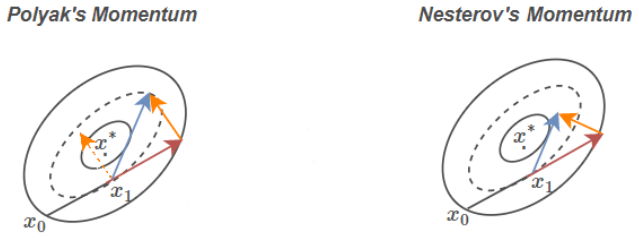
\includegraphics[scale=0.5]{img/momentum.png}
  	\caption{Polyak's and Nesterov's Momentum}
  	\label{fig:momentum}
\end{figure}

\begin{algorithm}[H]
	\caption{Polyak Accelerated Gradient Descent or or Heavy-Ball method}
	\label{alg:hbg}
	\begin{algorithmic}
		\Require{Function $f$ to minimize}
		\Require{Learning rate or step size $\alpha > 0$}
		\Require{Momentum $\beta \in [0,1)$}
		\Function{PolyakAcceleratedGradientDescent}{$f,\alpha,\beta$}
			\State Initialize weight vector $x_1 \gets x_0$ and velocity vector $v_0 \gets 0$
			\State $t \gets 1$
			\While{$not\_convergence$}
				\State $v_t = \beta v_{t-1} + \alpha \nabla f(x_t)$
				\State $x_{t+1} = x_t - v_t$
				\State $t \gets t + 1$
			\EndWhile
			\State \Return $x_t$
		\EndFunction
	\end{algorithmic}
\end{algorithm}

Leveraging the idea of momentum introduced by Polyak, Nesterov introduced a slightly altered update rule that has been shown to converge not only for quadratic functions, but for general convex functions. In the Nesterov's method \cite{nesterov1998introductory}, instead, the velocity vector $v_t$ is calculated by applying the $\beta$ momentum to the previous $v_{t-1}$ displacement, and subtracting the gradient step to $x_t + \beta v_{t-1}$, which is the point where the momentum term leads from $x_t$.

\begin{algorithm}[H]
	\caption{Nesterov Accelerated Gradient Descent}
	\label{alg:nag}
	\begin{algorithmic}
		\Require{Function $f$ to minimize}
		\Require{Learning rate $\alpha > 0$}
		\Require{Momentum $\beta \in [0,1)$}
		\Function{NesterovAcceleratedGradientDescent}{$f,\alpha,\beta$}
			\State Initialize weight vector $x_1 \gets x_0$ and velocity vector $v_0 \gets 0$
			\State $t \gets 1$
			\While{$not\_convergence$}
				\State $\hat{x}_t \gets x_t + \beta v_{t-1}$
				\State $v_t \gets \beta v_{t-1} + \alpha \nabla f(\hat{x}_t)$
				\State $x_{t+1} \gets x_t - v_t$
				\State $t \gets t + 1$
			\EndWhile
			\State \Return $x_t$
		\EndFunction
	\end{algorithmic}
\end{algorithm}

Comparing the algorithm \ref{alg:hbg} with the algorithm \ref{alg:nag}, we can see that Polyak’s method evaluates the gradient before adding momentum, whereas Nesterov’s algorithm evaluates it after applying momentum, which intuitively brings us closer to the minimum $x^*$, as showb in figure \ref{fig:momentum}.

Nesterov momentum brings the rate of convergence from $\displaystyle \mathcal{O}\Big(\frac{1}{t}\Big)$ to $\displaystyle \mathcal{O}\Big(\frac{1}{t^2}\Big)$ and in the case of smooth and strongly convex functions gives the acceleration that we had with Polyak’s momentum for quadratic functions. This is great, because we get the guarantee for a more general class of functions.

\bigskip

We can write the iteration complexity of these methods, i.e., the smallest $t$ such that we’re within $\epsilon$, for a L-smooth and $\mu$-strongly convex function as $\displaystyle \mathcal{O}\Big(\kappa \log \frac{1}{\epsilon}\Big)$ for the standard GD method, $\displaystyle \mathcal{O}\Big(\sqrt{\kappa}\log \frac{1}{\epsilon}\Big)$ for the Polyak’s method and, finally, $\displaystyle \mathcal{O}\Big(\frac{1}{\sqrt{\epsilon}}\Big)$ for the NAG method to get $\epsilon$-close to global optimum and where $\kappa$, i.e., the \emph{conditioning number}, is defined as $\kappa = L/\mu$ and where $L$ and $\mu$ are also equal to the smallest and the largest eigenvalues $\lambda_{min}$ and $\lambda_{max}$ respectively.

\pagebreak

\subsection{AdaGrad}

Due to the sparsity of the weight vector of the \emph{Lagrangian dual}, i.e., the Lagrange multipliers, we might end up in a situation where some components of the gradient are very small and others large. This, in terms of \emph{conditioning number}, i.e., $\kappa = L/\mu \gg 1$, means that the level sets of $f$ are ellipsoid, i.e., we are dealing with an ill-conditioned problem. So, given a learning rate, a standard gradient descent approach might end up in a situation where it decreases too quickly the small weights or too slowly the large ones.

Another method, that is usually deprecated in ML applications due to its increased computational complexity, is Newton’s method. Newton’s method favors a much faster convergence rate, i.e., number of iterations, at the cost of being more expensive per iteration. For convex problems, the recursion is similar to the gradient descent algorithm:

$$
x_{t+1} = x_t - \alpha H^{-1} \nabla f(x_t)
$$

where $\alpha$ is often close to one (damped-Newton) or one, and $H^{-1}$ denotes the Hessian of $f$ at the current point, i.e., $\nabla^2 f(x_t)$.

The above suggest a general rule in optimization: find any preconditioner, in convex optimization it has to be positive semidefinite, that improves the performance of gradient descent in terms of iterations, but without wasting too much time to compute that precoditioner. The above result into:

$$
x_{t+1} = x_t - \alpha P^{-1} \nabla f(x_t)
$$

where $P$ is the preconditioner. This idea is the basis of the BFGS quasi-Newton method.

The \emph{AdaGrad} \cite{duchi2011adaptive} algorithm is just a variant of preconditioned gradient descent, where $P$ is selected to be a diagonal preconditioner matrix and is updated using the gradient information, in particular it is the diagonal approximation of the inverse of the square roots of gradient outer products, until the $k$-th iteration. The above lead to the algorithm:

\begin{algorithm}[H]
	\caption{AdaGrad}
	\label{alg:adagrad}
	\begin{algorithmic}
		\Require{Function $f$ to minimize}
		\Require{Learning rate or step size $\alpha > 0$}
		\Require{Offset $\epsilon > 0$ to ensures not divide by 0}
		\Function{AdaGrad}{$f,\alpha,\epsilon$}
			\State Initialize weight vector $x_0$ and the squared accumulated gradients vector $s_t \gets 0$
			\State $t = 1$
			\While {$not\_convergence$}
				\State $g_t \gets \nabla f(x_t)$
				\State $s_t \gets s_{t-1} + g_t^2$
				\State $x_{t+1} \gets x_t - \alpha P^{-1} g_t = x_t - \displaystyle \frac{\alpha}{\sqrt{s_t + \epsilon}} \odot g_t \ \text{where} \ P \gets diag(s_t + \epsilon)^{1/2}$
				\State $t \gets t + 1$
			\EndWhile
			\State \Return $x_t$
		\EndFunction
	\end{algorithmic}
\end{algorithm}

In practical terms, \emph{AdaGrad} addresses the problem of the sparse optimal by adaptively scaling the learning rate for each dimension with the magnitude of the gradients. Coordinates that routinely correspond to large gradients are scaled down significantly, whereas others with small gradients receive a much more gentle treatment. \emph{AdaGrad}'s convergence rate for L-smooth convex functions is $\displaystyle \mathcal{O}\Big(\frac{1}{\sqrt{t}}\Big)$.

\pagebreak

\subsection{Sequential Minimal Optimization}

The \emph{Sequential Minimal Optimization (SMO)} \cite{platt1998sequential} method is the most popular approach for solving the SVM QP problem without any extra $Q$ matrix storage required by common QP methods. The advantage of SMO lies in the fact that it performs a series of two-point optimizations since we deal with just one equality constraint, so the Lagrange multipliers can be solved analitically.

\subsubsection{Classification}

At each iteration, SMO chooses two $\alpha_i$ to jointly optimize, let $\alpha_1$ and $\alpha_2$, finds the optimal values for these multipliers and update the SVM to reflect these new values. In order to solve for two Lagrange multipliers, SMO first computes the constraints over these and then solves for the constrained minimum. Since there are only two multipliers, the box-constraints cause the Lagrange multipliers to lie within a box, while the linear equality constraint causes the Lagrange multipliers to lie on a diagonal line inside the box. So, the constrained minimum must lie there as shown in \ref{fig:smo_lagrange_multipliers}.

\begin{figure}[h!]
	\centering
	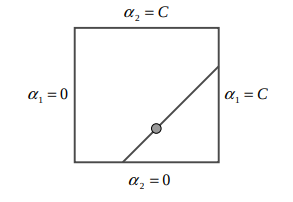
\includegraphics[scale=0.5]{img/smo_multipliers.png}
	\caption{SMO for two Lagrange multipliers}
	\label{fig:smo_lagrange_multipliers}
\end{figure}

In case of classification the ends of the diagonal line segment, i.e., the lower and upper bounds, can be espressed as follow if the target $y_1 \ne y_2$:

\begin{equation} \label{eq:smo_svc_bounds_update1}
	\begin{aligned}
		& L = max(0, \alpha_2 - \alpha_1) \\
		& H = min(C, C + \alpha_2 - \alpha_1)
	\end{aligned}
\end{equation}

or, alternatively, if the target $y_1 = y_2$:

\begin{equation} \label{eq:smo_svc_bounds_update2}
	\begin{aligned}
		& L = max(0, \alpha_2 + \alpha_1 - C) \\
		& H = min(C, \alpha_2 + \alpha_1)
	\end{aligned}
\end{equation}

The second derivative of the objective quadratic function along the diagonl line can be expressed as:

\begin{equation} \label{eq:smo_eta}
	\eta = K(x_1, x_1) + K(x_2, x_2) - 2K(x_1, x_2)
\end{equation}

that will be grather than zero if the kernel matrix will be positive definite, so there will be a minimum along the linear equality constraints that will be:

\begin{equation} \label{eq:smo_svc_a2_new}
	\alpha_2^{new} = \alpha_2 + \frac{y_2(E_1 - E_2)}{\eta}
\end{equation}

where $E_i = y_i - y'_i$ is the error on the $i$-th training example and $y'_i$ is the output of the SVC for the same.

Then, the box-constrained minimum is found by clipping the unconstrained minimum to the ends of the line segment:

\begin{equation} \label{eq:smo_svc_a2_new_clipped}
    \alpha_2^{new,clipped} =
        \begin{cases}
            H & \text{if} \ \alpha_2^{new} \geq H \\
            \alpha_2^{new} & \text{if} \ L < \alpha_2^{new} < H \\
            L & \text{if} \ \alpha_2^{new} \leq L \\
        \end{cases}
\end{equation}

Finally, the value of $\alpha_1$ is computed from the new clipped $\alpha_2$ as:

\begin{equation} \label{eq:smo_svc_a1_new}
	\alpha_1^{new} = \alpha_1 + s (\alpha_2 - \alpha_2^{new,clipped})
\end{equation}

where $s = y_1 y_2$.

Since the \emph{Karush-Kuhn-Tucker} conditions are necessary and sufficient conditions for optimality of a positive definite QP problem and the KKT conditions for the classification problem \eqref{eq:svc_min_wolfe_dual} are:

\begin{equation} \label{eq:svc_smo_kkt}
	\begin{aligned}
		\alpha_i = 0 & \Leftrightarrow y_i y'_i \geq 1 \\
		0 < \alpha_i < C & \Leftrightarrow y_i y'_i = 1 \\
		\alpha_i = C & \Leftrightarrow y_i y'_i \leq 1
	\end{aligned}
\end{equation}

the steps described above will be iterate as long as there will be an example that violates them.

After optimizing $\alpha_1$ and $\alpha_2$, we select the threshold $b$ such that the KKT conditions are satisfied for $x_1$ and $x_2$. If, after optimization, $\alpha_1$ is not at the bounds, i.e., $0 < \alpha_1 < C$, then the following threshold $b_{up}$ is valid, since it forces the SVC to output $y_1$ when the input is $x_1$:

\begin{equation} \label{eq:smo_svc_b1}
	b_{up} = E_1 + y_1 (\alpha_1^{new} - \alpha_1) K(x_1,x_1) + y_2 (\alpha_2^{new,clipped} - \alpha_2) K(x_1,x_2) + b
\end{equation}

similarly, the following threshold $b_{low}$ is valid if $0 < \alpha_2 < C$:

\begin{equation} \label{eq:smo_svc_b2}
	b_{low} = E_2 + y_1 (\alpha_1^{new} - \alpha_1) K(x_1,x_2) + y_2 (\alpha_2^{new,clipped} - \alpha_2) K(x_2,x_2) + b
\end{equation}

If, after optimization, both $0 < \alpha_1 < C$ and $0 < \alpha_2 < C$ then both these thresholds are valid, and they will be equal; else, if both $\alpha_1$ and $\alpha_2$ are at the bounds, i.e., $\alpha_1 = 0$ or $\alpha_1 = C$ and $\alpha_2 = 0$ or $\alpha_2 = C$, then all the thresholds between $b_{up}$ and $b_{low}$ satisfy the KKT conditions, so we choose the threshold to be halfway in between $b_{up}$ and $b_{low}$. This gives the complete equation for $b$:

\begin{equation} \label{eq:smo_svc_b}
	b =
        \begin{cases}
            b_{up} & \text{if} \ 0 < \alpha_1 < C \\
            b_{low} & \text{if} \ 0 < \alpha_2 < C \\
            \displaystyle \frac{b_{up}+b_{low}}{2} & \text{otherwise} \\
        \end{cases}
\end{equation}

\newpage

\begin{breakablealgorithm}
	\caption{Sequential Minimal Optimization for Classification}
	\label{alg:smo_classifier}
	\begin{algorithmic}
		\Require{Training examples matrix $X \in \Re^{n \times m}$}
		\Require{Training target vector $y \in \pm1^n$}
		\Require{Kernel matrix $K \in \Re^{n \times n}$}
		\Require{Regularization parameter $C > 0$}
		\Require{Tolerance value $tol$ for stopping criterion}
		\Function{SMOClassifier}{$X,y,K,C,tol$}
			\State Initialize the Lagrange multipliers vector $\alpha \in \Re^n, \alpha \gets 0$
			\State Initialize the empty set $I0 \gets \{i : 0 < \alpha_i < C\}$
			\State Initialize the set $I1 \gets \{i : y_i = +1, \alpha_i = 0\}$ to contain all the indices of the training examples of class $+1$
			\State Initialize the empty set $I2 \gets \{i : y_i = -1,	 \alpha_i = C\}$
			\State Initialize the empty set $I3 \gets \{i :  y_i = +1,	 \alpha_i = C\}$
			\State Initialize the set $I4 \gets \{i : y_i = -1, \alpha_i = 0\}$ to contain all the indices of the training examples of class $-1$
			\State Initialize $b_{up} \gets -1$
			\State Initialize $b_{low} \gets +1$
			\State Initialize the error cache vector $errors \in \Re^n, errors \gets 0$
			\While {$num\_changed > 0$ \OR $examine\_all = True$}
				\State $num\_changed \gets 0$
				\State $examine\_all \gets True$
				\If {$examine\_all = True$}
					\For {$i \gets 0$ to $n$} \Comment loop over all training examples
						\State $num\_changed \gets num\_changed + \Call{ExamineExample}{i}$
					\EndFor
				\Else
					\For {$i$ in $I0$} \Comment loop over examples where $\alpha_i$ are not already at their bounds
						\State $num\_changed \gets num\_changed + \Call{ExamineExample}{i}$
						\If {$b_{up} > b_{low} - 2 tol$} \Comment check if optimality on $I0$ is attained
							\State {$num\_changed \gets 0$}
							\Break
						\EndIf
					\EndFor
				\EndIf
				\If {$examine\_all = True$}
					\State $examine\_all \gets False$
				\ElsIf {$num\_changed = 0$}
					\State $examine\_all \gets True$
				\EndIf
			\EndWhile
			\State Compute $b$ by \eqref{eq:smo_svc_b}
			\State \Return $\alpha,b$
		\EndFunction
	\end{algorithmic}
	
	\newpage
	
	\begin{algorithmic}
		\Require{$i2$-th Lagrange multiplier}
		\Function{ExamineExample}{$i2$}
			\If {$i2$ in $I0$}
				\State $E_2 \gets errors_{i2}$
			\Else 
				\State Compute $E_2$
				\State $errors_{i2} \gets E_2$
				\State Update $(b_{low}, i_{low})$ or $(b_{up}, i_{up})$ using $(E_2, i2)$
			\EndIf
			\If {optimality is attained using current $b_{low}$ and $b_{up}$}
				\State \Return 0
			\Else
				\State Find an index $i1$ to do joint optimization with $i2$
				\If {$\Call{TakeStep}{i1,i2}$ = True}
					\State \Return 1
				\Else
					\State \Return 0
				\EndIf
			\EndIf
		\EndFunction
	\end{algorithmic}
	
	\newpage
	
	\begin{algorithmic}
		\Require{$i1$-th Lagrange multiplier}
		\Require{$i2$-th Lagrange multiplier}
		\Function{TakeStep}{$i1,i2$}
			\If {$i1 = i2$}
				\State \Return False
			\EndIf
			\State Compute $L$ and $H$ using \eqref{eq:smo_svc_bounds_update1} or \eqref{eq:smo_svc_bounds_update2}
			\If {$L = H$}
				\State \Return False
			\EndIf
			\State Compute $\eta$ by \eqref{eq:smo_eta} \Comment we assume that $\eta > 0$, i.e., the kernel matrix $K$ is positive definite
			\If {$\eta < 0$}
				\State Choose $\alpha_2^{new,clipped}$ between $L$ and $H$ according to the largest value of the objective function at these points
			\Else
				\State Compute $\alpha_2^{new}$ by \eqref{eq:smo_svc_a2_new}
				\State Compute $\alpha_2^{new,clipped}$ by \eqref{eq:smo_svc_a2_new_clipped}
			\EndIf
			\If {changes in $\alpha_2^{new,clipped}$ are larger than some eps}
				\State Compute $\alpha_1^{new}$ by \eqref{eq:smo_svc_a1_new}
				\State Update $\alpha_2^{new,clipped}$ and $\alpha_1^{new}$
				\For {$i$ in $I0$}
					\State Update $errors_i$ using new Lagrange multipliers
				\EndFor
				\State Update $\alpha$ using new Lagrange multipliers
				\State Update $I0, I1, I2, I3$ and $I4$
				\State Update $errors_{i1}$ and $errors_{i2}$
				\For {$i$ in $I0 \cup \{i1,i2\}$}
					\State Compute $(i_{low}, b_{low})$ by $b_{low} = \max\{errors_i : i \in I0 \cup I3 \cup I4\}$
					\State Compute $(i_{up}, b_{up})$ by $b_{up} = \min\{errors_i : i \in I0 \cup I1 \cup I2\}$
				\EndFor
				\State \Return True
			\Else
				\State \Return False
			\EndIf
		\EndFunction
	\end{algorithmic}
\end{breakablealgorithm}

\newpage

\subsubsection{Regression}

In case of regression the bounds and the new multipliers $\alpha_1^{+,new}$ and $\alpha_2^{+,new}$ can be espressed as follow if ($\alpha_1^+ > 0$ or ($\alpha_1^- = 0$ and $ E_1 - E_2 > 0$)) and ($\alpha_2^+ > 0$ or ($\alpha_2^- = 0$ and $ E_1 - E_2 < 0$)):

\begin{equation} \label{eq:smo_svr_bounds_update1}
	\begin{aligned}
		& L = max(0, \gamma - C) \\
		& H = min(C, \gamma)
	\end{aligned}
\end{equation}

\begin{equation} \label{eq:smo_svr_a2_new1}
	\alpha_2^{+,new} = \alpha_2^+ - \frac{E_1 - E_2}{\eta}
\end{equation}

\begin{equation} \label{eq:smo_svr_a1_new1}
	\alpha_1^{+,new} = \alpha_1^+ - (\alpha_2^{+,new,clipped} - \alpha_2^+)
\end{equation}

or, if ($\alpha_1^+ > 0$ or ($\alpha_1^- = 0$ and $ E_1 - E_2 > 2 \epsilon$)) and ($\alpha_2^- > 0$ or ($\alpha_2^+ = 0$ and $ E_1 - E_2 > 2 \epsilon$)):

\begin{equation} \label{eq:smo_svr_bounds_update2}
	\begin{aligned}
		& L = max(0, -\gamma) \\
		& H = min(C, -\gamma + C)
	\end{aligned}
\end{equation}

\begin{equation} \label{eq:smo_svr_a2_new2}
	\alpha_2^{-,new} = \alpha_2^- + \frac{(E_1 - E_2) - 2 \epsilon}{\eta}
\end{equation}

\begin{equation} \label{eq:smo_svr_a1_new2}
	\alpha_1^{+,new} = \alpha_1^+ + (\alpha_2^{-,new,clipped} - \alpha_2^-)
\end{equation}

or, if ($\alpha_1^- > 0$ or ($\alpha_1^+ = 0$ and $ E_1 - E_2 < - 2 \epsilon$)) and ($\alpha_2^+ > 0$ or ($\alpha_2^- = 0$ and $ E_1 - E_2 < - 2 \epsilon$)):

\begin{equation} \label{eq:smo_svr_bounds_update3}
	\begin{aligned}
		& L = max(0, \gamma) \\
		& H = min(C, C + \gamma)
	\end{aligned}
\end{equation}

\begin{equation} \label{eq:smo_svr_a2_new3}
	\alpha_2^{+,new} = \alpha_2^+ - \frac{(E_1 - E_2) + 2 \epsilon}{\eta}
\end{equation}

\begin{equation} \label{eq:smo_svr_a1_new3}
	\alpha_1^{-,new} = \alpha_1^- + (\alpha_2^{+,new,clipped} - \alpha_2^+)
\end{equation}

or, finally, if ($\alpha_1^- > 0$ or ($\alpha_1^+ = 0$ and $ E_1 - E_2 < 0$)) and ($\alpha_2^- > 0$ or ($\alpha_2^+ = 0$ and $ E_1 - E_2 > 0$)):

\begin{equation} \label{eq:smo_svr_bounds_update4}
	\begin{aligned}
		& L = max(0, -\gamma - C) \\
		& H = min(C, -\gamma)
	\end{aligned}
\end{equation}

\begin{equation} \label{eq:smo_svr_a2_new4}
	\alpha_2^{-,new} = \alpha_2^- + \frac{E_1 - E_2}{\eta}
\end{equation}

\begin{equation} \label{eq:smo_svr_a1_new4}
	\alpha_1^{-,new} = \alpha_1^- - (\alpha_2^{-,new,clipped} - \alpha_2^-)
\end{equation}

where $\gamma = \alpha_1^+ - \alpha_1^- + \alpha_2^+ - \alpha_2^-$. Notice that $\eta$ and $\alpha_2^{+,new,clipped}$ or $\alpha_2^{-,new,clipped}$ are identical to \eqref{eq:smo_eta} and \eqref{eq:smo_svc_a2_new_clipped} respectively.

The KKT conditions for the regression problem \eqref{eq:svr_min_wolfe_dual} are:

\begin{equation} \label{eq:svr_smo_kkt}
	\begin{aligned}
		\alpha_i^+ - \alpha_i^- = 0 & \Leftrightarrow | y_i - y'_i | < \epsilon \\
		-C < \alpha_i^+ - \alpha_i^- < C & \Leftrightarrow | y_i - y'_i | = \epsilon \\
		\alpha_i^+ + \alpha_i^- = C & \Leftrightarrow | y_i - y'_i | > \epsilon	
	\end{aligned}
\end{equation}

so, the steps described above will be iterate as long as there will be an example that violates them.

In case of regression we select the threshold $b$ as follows:

\begin{equation} \label{eq:smo_svr_b1}
	b_{up} = E_1 + ((\alpha_1^+ - \alpha_1^-) - (\alpha_1^{+,new} - \alpha_1^{-,new})) K(x_1,x_1) + ((\alpha_2^+ - \alpha_2^-) - (\alpha_2^{+,new,clipped} - \alpha_2^{-,new,clipped})) K(x_1,x_2) + b
\end{equation}

\begin{equation} \label{eq:smo_svr_b2}
	b_{low} = E_2 + ((\alpha_1^+ - \alpha_1^-) - (\alpha_1^{+,new} - \alpha_1^{-,new})) K(x_1,x_2) + ((\alpha_2^+ - \alpha_2^-) - (\alpha_2^{+,new,clipped} - \alpha_2^{-,new,clipped})) K(x_2,x_2) + b
\end{equation}

\begin{equation} \label{eq:smo_svr_b}
	b =
        \begin{cases}
            b_{up} & \text{if} \ 0 < \alpha_1^+, \alpha_1^- < C \\
            b_{low} & \text{if} \ 0 < \alpha_2^+, \alpha_2^- < C \\
            \displaystyle \frac{b_{up}+b_{low}}{2} & \text{otherwise} \\
        \end{cases}
\end{equation}

\bigskip
\bigskip

The improvements described in \cite{keerthi2001improvements, shevade1999improvements} for classification and regression respectively are about the definition of subsets of multipliers to efficiently update them at each iteration by separating the multipliers at the bounds from those who can be further minimized.

\newpage

\begin{breakablealgorithm}
	\caption{Sequential Minimal Optimization for Regression}
	\label{alg:smo_regression}
	\begin{algorithmic}
		\Require{Training examples matrix $X \in \Re^{n \times m}$}
		\Require{Training target vector $y \in \Re^n$}
		\Require{Kernel matrix $K \in \Re^{n \times n}$}
		\Require{Regularization parameter $C > 0$}
		\Require{Epsilon-tube value $\epsilon \geq 0$ within which no penalty is associated in the epsilon-insensitive loss function}
		\Require{Tolerance value $tol$ for stopping criterion}
		\Function{SMORegression}{$X,y,K,C,\epsilon,tol$}
			\State Initialize the Lagrange multipliers vector $\alpha^+ \in \Re^n, \alpha^+ \gets 0$
			\State Initialize the Lagrange multipliers vector $\alpha^- \in \Re^n, \alpha^- \gets 0$
			\State Initialize the empty set $I0 \gets \{i : 0 < \alpha^+_i, \alpha^-_i < C\}$
			\State Initialize the set $I1 \gets \{i : \alpha^+_i = 0, \alpha^-_i = 0\}$ to contain all the indices of the training examples
			\State Initialize the empty set $I2 \gets \{i : \alpha^+_i = 0, \alpha^-_i = C\}$
			\State Initialize the empty set $I3 \gets \{i : \alpha^+_i = C, \alpha^-_i = 0\}$
			\State Initialize $i_{up} \gets 0$ \Comment or any other target index $i_{up}$ from the training examples
			\State Initialize $i_{low} \gets 0$ \Comment or any other target index $i_{low}$ from the training examples
			\State Initialize $b_{up} \gets y_{i_{up}} + \epsilon$
			\State Initialize $b_{low} \gets y_{i_{low}} - \epsilon$
			\State Initialize the error cache vector $errors \in \Re^n, errors \gets 0$
			\While {$num\_changed > 0$ \OR $examine\_all = True$}
				\State $num\_changed \gets 0$
				\State $examine\_all \gets True$
				\If {$examine\_all = True$}
					\For {$i \gets 0$ to $n$} \Comment loop over all training examples
						\State $num\_changed \gets num\_changed + \Call{ExamineExample}{i}$
					\EndFor
				\Else
					\For {$i$ in $I0$} \Comment loop over examples where $\alpha^+_i$ and $\alpha^-_i$ are not already at their bounds
						\State $num\_changed \gets num\_changed + \Call{ExamineExample}{i}$
						\If {$b_{up} > b_{low} - 2 tol$} \Comment check if optimality on $I0$ is attained
							\State {$num\_changed \gets 0$}
							\Break
						\EndIf
					\EndFor
				\EndIf
				\If {$examine\_all = True$}
					\State $examine\_all \gets False$
				\ElsIf {$num\_changed = 0$}
					\State $examine\_all \gets True$
				\EndIf
			\EndWhile
			\State Compute $b$ by \eqref{eq:smo_svr_b}
			\State \Return $\alpha^+,\alpha^-,b$
		\EndFunction
	\end{algorithmic}
	
	\newpage
	
	\begin{algorithmic}
		\Require{$i1$-th Lagrange multiplier}
		\Require{$i2$-th Lagrange multiplier}
		\Function{TakeStep}{$i1,i2$}
			\If {$i1 = i2$}
				\State \Return False
			\EndIf
			\State $finished = False$
			\While {\NOT $finished$}
				\State Compute $L$ and $H$ using \eqref{eq:smo_svr_bounds_update1}, \eqref{eq:smo_svr_bounds_update2}, \eqref{eq:smo_svr_bounds_update3} or \eqref{eq:smo_svr_bounds_update4}
				\If {$L < H$}
					\State Compute $\eta$ by \eqref{eq:smo_eta} \Comment we assume that $\eta > 0$, i.e., the kernel matrix $K$ is positive definite
					\If {$\eta < 0$}
						\State Choose $\alpha_2^{+,new,clipped}$ or $\alpha_2^{-,new,clipped}$ between $L$ and $H$ according to the largest value of the objective function at these points
					\Else
						\State Compute $\alpha_2^{+,new}$ or $\alpha_2^{-,new}$ using \eqref{eq:smo_svr_a2_new1}, \eqref{eq:smo_svr_a2_new3} or \eqref{eq:smo_svr_a2_new2}, \eqref{eq:smo_svr_a2_new4} respectively
						\State Compute $\alpha_2^{+,new,clipped}$ or $\alpha_2^{-,new,clipped}$ by \eqref{eq:smo_svc_a2_new_clipped}
					\EndIf
					\State Compute $\alpha_1^{+,new}$ or $\alpha_1^{-,new}$ using \eqref{eq:smo_svr_a1_new1}, \eqref{eq:smo_svr_a1_new2} or \eqref{eq:smo_svr_a1_new3}, \eqref{eq:smo_svr_a1_new4} respectively
					\If {changes in $\alpha_2^{+,new,clipped}, \alpha_2^{-,new,clipped}, \alpha_1^{+,new}$ or $\alpha_1^{-,new}$ are larger than some eps}
						\State Update $\alpha_2^{+,new,clipped}, \alpha_2^{-,new,clipped}, \alpha_1^{+,new}$ or $\alpha_1^{-,new}$
					\EndIf
				\Else
					\State $finished = True$
				\EndIf
			\EndWhile
			\If {changes in $\alpha_2^{+,new,clipped}, \alpha_2^{-,new,clipped}, \alpha_1^{+,new}$ or $\alpha_1^{-,new}$ are larger than some eps}
				\For {$i$ in $I0$}
					\State Update $errors_i$ using new Lagrange multipliers
				\EndFor
				\State Update $\alpha^+$ and $\alpha^-$ using new Lagrange multipliers
				\State Update $I0, I1, I2$ and $I3$
				\State Update $errors_{i1}$ and $errors_{i2}$
				\For {$i$ in $I0 \cup \{i1,i2\}$}
					\State Compute $(i_{low}, b_{low})$ by $b_{low} = \max\{errors_i : i \in I0 \cup I1 \cup I2\}$
					\State Compute and $(i_{up}, b_{up})$ by $b_{up} = \min\{errors_i : i \in I0 \cup I1 \cup I3\}$
				\EndFor
				\State \Return True
			\Else
				\State \Return False
			\EndIf
		\EndFunction
	\end{algorithmic}
\end{breakablealgorithm}